\documentclass[final,12pt]{elsarticle}
\usepackage{amssymb}
\usepackage{amsmath}
\usepackage{tikz}

\begin{document}

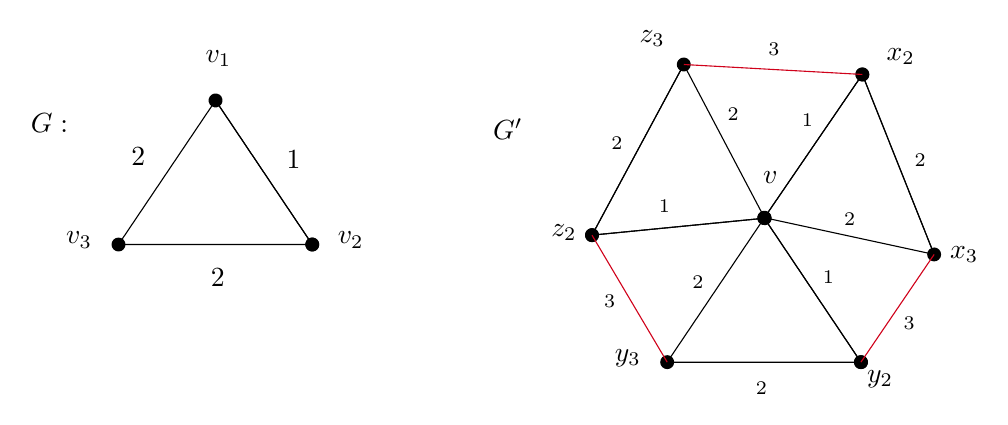
\begin{tikzpicture}[x=0.75pt,y=0.75pt,yscale=-0.85,xscale=0.85]

\draw   (139.17,59.33) -- (194,141) -- (84.17,141) -- cycle ;
\draw    (139.17,59.33) -- (194,141) ;
\draw [shift={(194,141)}, rotate = 56.12] [color={rgb, 255:red, 0; green, 0; blue, 0 }  ][fill={rgb, 255:red, 0; green, 0; blue, 0 }  ][line width=0.75]      (0, 0) circle [x radius= 3.35, y radius= 3.35]   ;
\draw [shift={(139.17,59.33)}, rotate = 56.12] [color={rgb, 255:red, 0; green, 0; blue, 0 }  ][fill={rgb, 255:red, 0; green, 0; blue, 0 }  ][line width=0.75]      (0, 0) circle [x radius= 3.35, y radius= 3.35]   ;
\draw    (194,141) -- (84.17,141) ;
\draw [shift={(84.17,141)}, rotate = 180] [color={rgb, 255:red, 0; green, 0; blue, 0 }  ][fill={rgb, 255:red, 0; green, 0; blue, 0 }  ][line width=0.75]      (0, 0) circle [x radius= 3.35, y radius= 3.35]   ;
\draw [shift={(194,141)}, rotate = 180] [color={rgb, 255:red, 0; green, 0; blue, 0 }  ][fill={rgb, 255:red, 0; green, 0; blue, 0 }  ][line width=0.75]      (0, 0) circle [x radius= 3.35, y radius= 3.35]   ;
\draw   (450.17,126) -- (505,207.67) -- (395.17,207.67) -- cycle ;
\draw    (450.17,126) -- (505,207.67) ;
\draw [shift={(505,207.67)}, rotate = 56.12] [color={rgb, 255:red, 0; green, 0; blue, 0 }  ][fill={rgb, 255:red, 0; green, 0; blue, 0 }  ][line width=0.75]      (0, 0) circle [x radius= 3.35, y radius= 3.35]   ;
\draw [shift={(450.17,126)}, rotate = 56.12] [color={rgb, 255:red, 0; green, 0; blue, 0 }  ][fill={rgb, 255:red, 0; green, 0; blue, 0 }  ][line width=0.75]      (0, 0) circle [x radius= 3.35, y radius= 3.35]   ;
\draw    (505,207.67) -- (421.17,207.67) -- (395.17,207.67) ;
\draw [shift={(395.17,207.67)}, rotate = 180] [color={rgb, 255:red, 0; green, 0; blue, 0 }  ][fill={rgb, 255:red, 0; green, 0; blue, 0 }  ][line width=0.75]      (0, 0) circle [x radius= 3.35, y radius= 3.35]   ;
\draw [shift={(505,207.67)}, rotate = 180] [color={rgb, 255:red, 0; green, 0; blue, 0 }  ][fill={rgb, 255:red, 0; green, 0; blue, 0 }  ][line width=0.75]      (0, 0) circle [x radius= 3.35, y radius= 3.35]   ;
\draw   (450.26,125.8) -- (505.79,44.6) -- (546.49,146.62) -- cycle ;
\draw    (450.26,125.8) -- (505.79,44.6) ;
\draw [shift={(505.79,44.6)}, rotate = 304.37] [color={rgb, 255:red, 0; green, 0; blue, 0 }  ][fill={rgb, 255:red, 0; green, 0; blue, 0 }  ][line width=0.75]      (0, 0) circle [x radius= 3.35, y radius= 3.35]   ;
\draw [shift={(450.26,125.8)}, rotate = 304.37] [color={rgb, 255:red, 0; green, 0; blue, 0 }  ][fill={rgb, 255:red, 0; green, 0; blue, 0 }  ][line width=0.75]      (0, 0) circle [x radius= 3.35, y radius= 3.35]   ;
\draw    (505.79,44.6) -- (546.49,146.62) ;
\draw [shift={(546.49,146.62)}, rotate = 68.25] [color={rgb, 255:red, 0; green, 0; blue, 0 }  ][fill={rgb, 255:red, 0; green, 0; blue, 0 }  ][line width=0.75]      (0, 0) circle [x radius= 3.35, y radius= 3.35]   ;
\draw [shift={(505.79,44.6)}, rotate = 68.25] [color={rgb, 255:red, 0; green, 0; blue, 0 }  ][fill={rgb, 255:red, 0; green, 0; blue, 0 }  ][line width=0.75]      (0, 0) circle [x radius= 3.35, y radius= 3.35]   ;
\draw   (450.44,126.08) -- (352.55,135.69) -- (404.57,38.96) -- cycle ;
\draw    (450.44,126.08) -- (352.55,135.69) ;
\draw [shift={(352.55,135.69)}, rotate = 174.39] [color={rgb, 255:red, 0; green, 0; blue, 0 }  ][fill={rgb, 255:red, 0; green, 0; blue, 0 }  ][line width=0.75]      (0, 0) circle [x radius= 3.35, y radius= 3.35]   ;
\draw [shift={(450.44,126.08)}, rotate = 174.39] [color={rgb, 255:red, 0; green, 0; blue, 0 }  ][fill={rgb, 255:red, 0; green, 0; blue, 0 }  ][line width=0.75]      (0, 0) circle [x radius= 3.35, y radius= 3.35]   ;
\draw    (352.55,135.69) -- (404.57,38.96) ;
\draw [shift={(404.57,38.96)}, rotate = 298.27] [color={rgb, 255:red, 0; green, 0; blue, 0 }  ][fill={rgb, 255:red, 0; green, 0; blue, 0 }  ][line width=0.75]      (0, 0) circle [x radius= 3.35, y radius= 3.35]   ;
\draw [shift={(352.55,135.69)}, rotate = 298.27] [color={rgb, 255:red, 0; green, 0; blue, 0 }  ][fill={rgb, 255:red, 0; green, 0; blue, 0 }  ][line width=0.75]      (0, 0) circle [x radius= 3.35, y radius= 3.35]   ;
\draw [color={rgb, 255:red, 208; green, 2; blue, 27 }  ,draw opacity=1 ]   (352.55,135.69) -- (395.17,207.67) ;
\draw [color={rgb, 255:red, 208; green, 2; blue, 27 }  ,draw opacity=1 ]   (546.49,146.62) -- (505,207.67) ;
\draw [color={rgb, 255:red, 208; green, 2; blue, 27 }  ,draw opacity=1 ]   (404.57,38.96) -- (505.79,44.6) ;

% Text Node
\draw (33,65.4) node [anchor=north west][inner sep=0.75pt]    {$G:$};
% Text Node
\draw (132,29.4) node [anchor=north west][inner sep=0.75pt]    {$v_{1}$};
% Text Node
\draw (207,132.4) node [anchor=north west][inner sep=0.75pt]    {$v_{2}$};
% Text Node
\draw (53,132.4) node [anchor=north west][inner sep=0.75pt]    {$v_{3}$};
% Text Node
\draw (507,211.07) node [anchor=north west][inner sep=0.75pt]    {$y_{2}$};
% Text Node
\draw (364,199.07) node [anchor=north west][inner sep=0.75pt]    {$y_{3}$};
% Text Node
\draw (518,28.4) node [anchor=north west][inner sep=0.75pt]    {$x_{2}$};
% Text Node
\draw (554,140.4) node [anchor=north west][inner sep=0.75pt]    {$x_{3}$};
% Text Node
\draw (378,18.4) node [anchor=north west][inner sep=0.75pt]    {$z_{3}$};
% Text Node
\draw (328,128.4) node [anchor=north west][inner sep=0.75pt]    {$z_{2}$};
% Text Node
\draw (448,98.4) node [anchor=north west][inner sep=0.75pt]    {$v$};
% Text Node
\draw (178,86.4) node [anchor=north west][inner sep=0.75pt]    {$1$};
% Text Node
\draw (135,153.4) node [anchor=north west][inner sep=0.75pt]    {$2$};
% Text Node
\draw (90,84.4) node [anchor=north west][inner sep=0.75pt]    {$2$};
% Text Node
\draw (295,68.4) node [anchor=north west][inner sep=0.75pt]    {$G'$};
% Text Node
\draw (428,62.4) node [anchor=north west][inner sep=0.75pt]  [font=\scriptsize]  {$2$};
% Text Node
\draw (470,65.4) node [anchor=north west][inner sep=0.75pt]  [font=\scriptsize]  {$1$};
% Text Node
\draw (482,154.4) node [anchor=north west][inner sep=0.75pt]  [font=\scriptsize]  {$1$};
% Text Node
\draw (389,114.4) node [anchor=north west][inner sep=0.75pt]  [font=\scriptsize]  {$1$};
% Text Node
\draw (408,157.4) node [anchor=north west][inner sep=0.75pt]  [font=\scriptsize]  {$2$};
% Text Node
\draw (534,88.4) node [anchor=north west][inner sep=0.75pt]  [font=\scriptsize]  {$2$};
% Text Node
\draw (362,78.4) node [anchor=north west][inner sep=0.75pt]  [font=\scriptsize]  {$2$};
% Text Node
\draw (444,217.4) node [anchor=north west][inner sep=0.75pt]  [font=\scriptsize]  {$2$};
% Text Node
\draw (494,121.4) node [anchor=north west][inner sep=0.75pt]  [font=\scriptsize]  {$2$};
% Text Node
\draw (358,168.4) node [anchor=north west][inner sep=0.75pt]  [font=\scriptsize]  {$3$};
% Text Node
\draw (527.74,180.54) node [anchor=north west][inner sep=0.75pt]  [font=\scriptsize]  {$3$};
% Text Node
\draw (451,25.4) node [anchor=north west][inner sep=0.75pt]  [font=\scriptsize]  {$3$};

\end{tikzpicture}

\end{document}